\documentclass{article}

\usepackage{cancel}
\usepackage{amsmath}
\usepackage[includehead,nomarginpar]{geometry}
\usepackage{graphicx}
\usepackage{amsfonts} 
\usepackage{verbatim}
\usepackage{mathrsfs}  
\usepackage{lmodern}
\usepackage{braket}
\usepackage{bookmark}
\usepackage{fancyhdr}
\usepackage{romanbarpagenumber}
\usepackage{minted}
%\usepackage{subfig}
\usepackage[italian]{babel}
\usepackage{float}
%\usepackage{wrapfig}
%\usepackage[export]{adjustbox}
\allowdisplaybreaks

\setlength{\headheight}{12.0pt}
\addtolength{\topmargin}{-12.0pt}
\graphicspath{ {../Immagini/} }

\hypersetup{
    colorlinks=true,
    linkcolor=black,
}

\newsavebox{\tempbox} %{\raisebox{\dimexpr.5\ht\tempbox-.5\height\relax}}


\makeatother

\numberwithin{equation}{subsection}
\newcommand{\tageq}{\tag{\stepcounter{equation}\theequation}}
\AtBeginDocument{%
  \renewcommand{\figurename}{Fig.}
}
\fancypagestyle{link}{\fancyhf{}\renewcommand{\headrulewidth}{0pt}\fancyfoot[C]{Sorgente del file LaTeX disponibile al seguente link: \url{https://github.com/00Darxk/Basi-di-Dati/}}}

\begin{document}

\title{%
    \textbf{Basi di Dati}  \\ 
    \large Esercizi Svolti di Basi di Dati \\
    \textit{Anno Accademico: 2024/25}}
\author{\textit{Giacomo Sturm}}
\date{\textit{Dipartimento di Ingegneria Civile, Informatica e delle Tecnologie Aeronautiche \\
Università degli Studi ``Roma Tre"}}

\maketitle
\thispagestyle{link}

\clearpage


\pagestyle{fancy}
\fancyhead{}\fancyfoot{}
\fancyhead[C]{\textit{Basi di Dati - Università degli Studi ``Roma Tre"}}
\fancyfoot[C]{\thepage}
\pagenumbering{Roman}

\tableofcontents

\clearpage
\pagenumbering{arabic}

\section{Esercitazione del 7 Ottobre}

\subsection{Esercizio 1}

Si considerano le seguenti relazioni, senza valori nulli:
\begin{itemize}
    \item $R_1(\underline{A},B)$ con vincolo di integrità referenziale, tra $B$ e la chiave $D$ di $R_2$. Con cardinalità $M_1=500$;
    \item $R_2(\underline{D},E,F,G)$, con vincolo di integrità referenziale, tra $F$ e $G$ e la chiave $H,P$ di $R_3$. Con cardinalità $M_2=1000$;
    \item $R_3(\underline{H},\underline{P},Q)$, con cardinalità $M_3=200$.
\end{itemize}

Determinare la cardinalità (numero di ennuple) massima e minima delle seguenti relazioni derivate:

\subsubsection*{Domanda 1}

L'equi-join tra $R_3$ e $R_1$ sulla condizione $Q=A$:
\begin{equation*}
    R_3\Join_{Q=A}R_1
\end{equation*}
Non comprendendo alcun vincolo di integrità referenziale tra le dure relazioni, potrebbe non contenere alcuna ennupla, quindi avere una cardinalità minima pari a zero. 
Invece potrebbe contenere al massimo un numero di ennuple pari al numero di attributi $Q$ non nulli, quindi pari alla cardinalità di $R_3$, $M_3$. 

\begin{equation}
    M_{D_1}\in[0,M_3]
\end{equation}

\subsubsection*{Domanda 2}

La proiezione sulla chiave $H,P$ di $R_3$:
\begin{equation*}
    \pi_{H,P}(R_3)
\end{equation*}

Poiché coinvolge una chiave della relazione, questa relazione derivata conterra esattamente tutte le ennuple presenti nella relazione di partenza, quindi avrà una cardinalità sempre pari 
alla cardinalità di $R_3$, $M_3$: 

\begin{equation}
    M_{D_2}=M_3
\end{equation}

\subsubsection*{Domanda 3}

La proiezione sugli attributi $H$ e $Q$ di $R_3$:
\begin{equation*}
    \pi_{H,Q}(R_3)
\end{equation*}

Questi due attributi insieme non formano una superchiave, quindi potrebbero i valori potrebbero fra loro collassare, quindi produrre una singola ennupla di attributi distinti. Invece è 
possibile che questa relazione contenga tutte le ennuple distinte della relazione $R_3$, e quindi abbia una cardinalità massima pari a $M_3$:
\begin{equation}
    M_{D_3}\in[1,M_3]
\end{equation}

In generale quando una proiezione non coinvolge una superchiave dell'operando, è possibile, ma non garantito, che abbia lo stesso numero di ennuple dell'operando. L'unico discriminante in una proiezione è la presenza 
o meno della chiave, o superchiave, negli attributi considerati. 

\subsubsection*{Domanda 4}

L'equi-join tra $R_1$ ed $R_2$ sulla condizione $B=D$:
\begin{equation*}
    R_1\Join_{B=D}R_2
\end{equation*}
Gli attributi $B$ e la chiave $D$ rappresentano un vincolo di integrità referenziale tra $R_1$ ed $R_2$. Ciascuna ennupla di $R_1$ può essere estesa con una singola ennupla distanza di $R_2$, 
poiché si effettua il join sulla sua chiave. La cardinalità di questa relazione è quindi $M_1$.  
\begin{equation}
    M_{D_4}=M_1
\end{equation}

\subsubsection*{Domanda 5}

\begin{equation*}
    (R_1\Join_{B=D}R_2)\Join_{(F=H)\land(G=P)}R_3
\end{equation*}

Analogamente alla domanda precedente, poiché si effettua un join tra $R_3$ e la relazione precedente, su una chiave di $R_3$ ed un vincolo di integrità referenziale, allora la cardinalità 
corrisponde alla cardinalità dell'altro operando, calcolata nella domanda precedente pari a $M_1$:
\begin{equation}
    M_{D_5}=M_1
\end{equation}

\subsubsection*{Domanda 6}

L'equi-join tra $R_1$ ed $R_3$ su $B=H$:
\begin{equation*}
    R_1\Join_{B=H}R_3
\end{equation*}

Non sono presenti vincoli di integrità referenziale, o chiavi delle relazioni, quindi è possibile che non siano presenti ennuple, oppure che ogni ennupla della prima relazione, sia operata 
con ogni ennupla della seconda per un massimo di $M_1\cdot M_3$. Bisogna considerare che l'attributo $H$ non rappresenta una chiave primaria, quindi non si può effettuare lo stesso 
ragionamento della domanda 5. 
\begin{equation}
    M_{D_6}\in[0,M_1\cdot M_2]
\end{equation}

\subsubsection*{Domanda 7}

\begin{equation*}
    (R_1\Join_{B=D}R_2)\Join_{F=H}R_3
\end{equation*}

Il primo join interno ha cardinalità $M_1$, mentre nel secondo join, è presente solo una parte del vincolo di integrità referenziale. Quindi ogni ennupla del primo join può al minimo 
trovare una sua controparte in $R_3$, avendo una cardinalità minima di $M_1$. Mentre al massimo, non essendo completo il vincolo, è possibile che tutte le ennuple di $R_1$ siano combinate 
con tutte le ennuple di $R_3$:
\begin{equation}
    M_{D_7}\in[M_1,M_1\cdot M_3]
\end{equation}

\subsection{Esercizio 2}

Si considera la seguente \href{https://dbis-uibk.github.io/relax/calc/gist/b7a8eac38317e0d6a7f0b904a9a10bd3}{base di dati} su RelaX.

%% TODO img inserire alberi \sim RelaX

\subsubsection*{Domanda 1}

Trovare matricola, nome, età e stipendio degli impiegati che guadagnano più di 40. Si utilizza una semplice selezione sulla relazione impiegati, specificando la condizione di selezione, e non è necessario 
effettuare una proiezione, poiché si utilizzano tutti gli attributi: 

\begin{minted}[mathescape,escapeinside=||]{sql}
    |$\sigma$| Stipendio>40 (Impiegati)
\end{minted}

\subsubsection*{Domanda 2}

Trovare matricola, nome ed età degli impiegati che guadagnano più di 40. In questa interrogazione è necessario effettuare una proiezione sulla lista di attributi di interesse, dato il risultato alla precedente 
domanda:

\begin{minted}[mathescape, escapeinside=||]{sql}
    |$\pi$| Matricola, Nome, Eta (|$\sigma$| Stipendio>40 (Impiegati))
\end{minted}

\subsubsection*{Domanda 3}

Trovare le matricole dei capi che guadagnano più di 40. Si può effettuare prima sia il join che la selezione, ma discussione in termini di efficienza non vengono trattate in questo corso. Si effettua una selezione 
sullo stipendio, come per le prime due domande. Si effettua un join tra questa relazione e supervisione sulla condizione matricola, di impiegati, ed impiegato, di supervisione. Per ottenere solamente l'attributo 
richiesto si effettua una proiezione su capo:
\begin{minted}[mathescape, escapeinside=||]{sql}
    |$\pi$| Capo ( (Supervisione)
        |$\Join$| Matricola=Impiegato
        (|$\sigma$| Stipendio>40 (Impiegati))
    )
\end{minted}

Ovviamente quest'interrogazione produce un risultato solamente sui dati noti, in questa base di dati non sono presenti informazioni sui capi di alcuni impiegati, quindi non è possibile creare informazioni su di loro. 

\subsubsection*{Domanda 4}
Trovare nome e stipendio dei capi degli impiegati che guadagnano più di 40. Considerando i capi come impiegati, nella relazione impiegati sono presenti queste informazioni. Quindi dalla relazione precedente è possibile 
effettuare un join ulteriore con la relazione impiegati su \verb|Capo = Impiegato|, ed in seguito una selezione per identificare le informazioni di interesse:
\begin{minted}[mathescape, escapeinside=||]{sql}
    |$\pi$| Nome, Stipendio ( (Impiegati)
        |$\Join$| Impiegato=Capo 
            (|$\pi$| Capo ( (Supervisione)
                |$\Join$| Matricola=Impiegato
                (|$\sigma$| Stipendio>40 (Impiegati)))))
\end{minted}

\subsubsection*{Domanda 5}

Trovare gli impiegati che guadagnano più del proprio capo, mostrando matricola, nome e stipendio dell'impiegato e del capo. Per trovare questo risultato bisognerebbe utilizzare due copie della stessa relazione 
impiegati per confrontare gli stipendi del capo, e dell'impiegato. Ma per poter confrontare questi attributi bisognerebbe rinominare gli attributi di una delle due, prima del join tra di loro, per correlare 
le informazioni necessarie. Il join si effettua prima tra le matricole dei capi e supervisione e poi nuovamente con la relazione impiegati, per correlare per ogni impiegato, le informazioni del suo capo. A questo 
punto si può effettuare una selezione per rimuovere le ennuple dove il capo guadagna di più del proprio impiegato, ed una proiezione finale sugli attributi di interesse:

\begin{minted}[mathescape, escapeinside=||]{sql}
    |$\pi$| Matricola, Nome, Stipendio, MatricolaCapo, NomeCapo, StipendioCapo (
        |$\sigma$| Stipendio > StipendioCapo (
            (|$\rho$| MatricolaCapo |$\leftarrow$| Matricola, NomeCapo |$\leftarrow$| Nome, 
               StipendioCapo |$\leftarrow$| Stipendio, EtaCapo |$\leftarrow$| Eta (Impiegati))
            |$\Join$| MatricolaCapo=Capo
            ((Supervisione) |$\Join$| Matricola=Impiegato (Impiegati))))
\end{minted}


Questo processo è molto verboso, ed è possibile semplificarlo mediante l'utilizzo di viste. Utilizzano le viste si può rinominare la relazione impiegati a \verb|Capi|, per poter utilizzare la notazione puntate 
per riferirsi ai suoi attributi:
\begin{minted}[mathescape, escapeinside=||]{sql}
    Capi = |$\rho$| Capi (Impiegati) 

    |$\pi$| Impiegato.Matricola, Impiegato.Nome, Impiegato.Stipendio, 
      Capi.Matricola, Capi.Nome, Capi.Stipendio (
        |$\sigma$| Stipendio > Capi.Stipendio ((Capi)
            |$\Join$| Capi.Matricola=Capo
            ((Supervisione) |$\Join$| Matricola=Impiegato (Impiegati))))
\end{minted}

\subsubsection*{Domanda 6}

Trovare matricola, nome e stipendio dei capi degli impiegati che guadagnano più di 40; per ciascuno, mostrare, matricola, nome e stipendio anche dell'impiegato. Questa rappresenta una versione semplificata 
della domanda precedente, quindi invece di effettuare una selezione dopo il join tra capi ed impiegati, si effettua la selezione come per le domande precedenti:

\begin{minted}[mathescape, escapeinside=||]{sql}
    |$\pi$| Impiegato.Matricola, Impiegato.Nome, Impiegato.Stipendio, 
      Capi.Matricola, Capi.Nome, Capi.Stipendio (
        ((Capi) |$\Join$| Capi.Matricola=Capo
        ((Supervisione) |$\Join$| Matricola=Impiegato (|$\sigma$| Stipendio>40 (Impiegati)))))
\end{minted}

\subsubsection*{Domanda 7}

Trovare le matricole dei capi i cui impiegati guadagnano tutti più di 40. Quest'interrogazione è semplice, poiché è sufficiente individuare tutti i capi con almeno un impiegato che guadagna meno di 40, da togliere poi 
tramite una differenza tra insiemi alla vista capi. Rimangono sicuramente tutti i capi con impiegati che guadagnano più di 40:
\begin{minted}[mathescape, escapeinside=||]{sql}
    |$\pi$| Capo (Supervisione) -
    |$\pi$| Capo ((Supervisione) |$\Join$| Matricola=Impiegato
    (|$\sigma$| Stipendio|$\leq$|40 (Impiegati)))

\end{minted}

\clearpage

\section{Esercitazione del 18 e 25 Ottobre}


Si considera la seguente base di dati:
\begin{minted}{sql}
CREATE TABLE Compositori (codice integer NOT NULL PRIMARY KEY,
                        cognome text ,
                        nome text);
						
CREATE TABLE Concerti (codice integer NOT NULL PRIMARY KEY,
                        titolo text ,
                        descrizione text);

CREATE TABLE Pezzi (codice  integer NOT NULL PRIMARY KEY,
                        titolo text,
                        autore integer NOT NULL REFERENCES Compositori,
                        durata integer);

CREATE TABLE Programmazione ( pezzo integer NOT NULL REFERENCES Pezzi,
                        concerto integer NOT NULL REFERENCES Concerti, 
                        posizione integer,
                        PRIMARY KEY(pezzo, concerto));

\end{minted}

Popolato dai seguenti valori:
\begin{minted}{sql}
insert into compositori values(1, 'Mozart', 'Wolfgang Amadeus');
insert into compositori values(2, 'Bach', 'Johann Sebastian');
insert into compositori values(3, 'Beethoven', 'Ludwig van');

insert into concerti values(1, 'Concerto di Febbraio', 'Selezione di musica Barocca');
insert into concerti values(2, 'Concerto di Marzo', 'Estratti di belle sinfonie');
insert into concerti values(3, 'Concerto di Giugno', 'Concerto a Villa Ada');

insert into pezzi values(1, 'Variazioni Goldberg', 2, 32);
insert into pezzi values(2, 'L''arte della fuga', 2, 38);
insert into pezzi values(3, 'Il clavicembalo ben temperato', 2, 85);
insert into pezzi values(4, 'Il flauto magico', 1, 95);
insert into pezzi values(5, 'Serenata in do minore k 388', 1, 45);
insert into pezzi values(6, 'Requiem', 1, 87);
insert into pezzi values(7, 'Sinfonia n. 6 in fa maggiore op. 68', 3, 91);
insert into pezzi values(8, 'Sinfonia n. 9 in re minore', 3, 91);
insert into pezzi values(9, 'Trio d''archi in mi bemolle maggiore op. 3', 3, 52);

insert into programmazione values(1, 1,1);
insert into programmazione values(2, 1,2);
insert into programmazione values(3, 2,2);
insert into programmazione values(4, 3,1);
insert into programmazione values(5, 2,3);
insert into programmazione values(5, 3,2);
insert into programmazione values(7, 2,1);
\end{minted}

Vengono proposti una serie di esercizi su questo database. 

\subsection{Domanda 1}
Determinare il titolo dei pezzi che hanno durata compresa tra 40 e 60 minuti. Per effettuare quest'operazione è sufficiente operare sulla singola tabella \verb|Pezzi|:
\begin{minted}{sql}
SELECT titolo FROM Pezzi
WHERE durata>40 AND durata<60
\end{minted}

\subsection{Domanda 2}
Determinare il titolo, nome e cognome dell'autore dei pezzi che hanno durata compresa tra 40 e 60 minuti. Oltre alla tabella \verb|Pezzi|, è necessario ottenere i campi 
\verb|nome| e \verb|cognome| della tabella \verb|Compositori|. Si effettua mediante un join, specificando come vengono associate le due relazioni, infatti il campo \verb|autore| 
di \verb|Pezzi| si riferisce alla chiave primaria della relazione \verb|Compositori|:
\begin{minted}{sql}
SELECT titolo, nome, cognome  
FROM Pezzi JOIN Compositori ON Pezzi.autore=Compositori.codice
WHERE durata>40 and durata<60
\end{minted}

\subsection{Domanda 3}
Determinare il nome e cognome dei compositori dei pezzi presenti nel ``Concerto di Giugno''. Per ottenere questo si utilizza una vista. Nei database industriali 
la vista p contenuta nella cache. La vista può essere utilizzata come fosse un'altra tabella nel database, ed è possibile utilizzarla per effettuare altre 
interrogazioni nella stessa query. Si crea quindi una vista di tutti i pezzi presenti nel concerto di Giugno:
\begin{minted}{sql}
CREATE VIEW pezzi_giugno AS Select *
FROM Concerti JOIN Programmazione ON Concerti.codice=Programmazione.concerto
WHERE Concerti.titolo='Concerto di Giugno'
\end{minted}
Per ottenere il nome ed il cognome dei compositori si effettua una join su questa vista, prima con i pezzi, e poi con la relazione compositori, selezionando solo gli 
attributi richiesti:
\begin{minted}{sql}
SELECT DISTINCT nome, cognome
FROM pezzi_giugno JOIN Pezzi ON pezzi_giugno.pezzo=Pezzi.codice
JOIN Compositori ON Compositori.codice=autore
\end{minted}

\subsection{Domanda 4}
Determinare il nome e cognome dei compositori che non hanno pezzi nel ``Concerto di Giugno''. Utilizzando la stessa vista \verb|pezzi_giugno|, è possibile utilizzare una semplice \verb|EXCEPT| sulla 
relazione dei compositori per rimuovere quelli presenti nel concerto di Giugno:
\begin{minted}{sql}
SELECT DISTINCT nome, cognome
FROM Compositori EXCEPT
SELECT DISTINCT nome, cognome
FROM pezzi_giugno JOIN pezzi ON pezzo=pezzi.codice 
JOIN Compositori ON autore=Compositori.codice
\end{minted}

\subsection{Domanda 5}
Determinare il titolo e descrizione dei concerti in cui sono presenti pezzi di Mozart. Per ottenere questi risultati è sufficiente effettuare un'operazione di join tra tutte le relazioni del database, 
considerando solo le ennuple di valore specificato per l'attributo \verb|cognome|:
\begin{minted}{sql}
SELECT DISTINCT Concerti.titolo, descrizione 
FROM Concerti JOIN Programmazione ON Concerti.codice=Programmazione.concerto
JOIN pezzi ON pezzi.codice=pezzo
JOIN Compositori ON autore=Compositori.codice
WHERE cognome='Mozart'
\end{minted}

\subsection{Domanda 6}
Determinare il titolo e descrizione dei concerti in cui non sono presenti pezzi di Beethoven. Per effettuare quest'operazione è sufficiente trovare tutti i concerti dove sono presenti 
pezzi di Beethoven, come nella domanda precedente, ed in seguito rimuoverli dalla lista di tutti i concerti con un \verb|EXCEPT| iniziale:
\begin{minted}{sql}
SELECT DISTINCT concerti.titolo, descrizione
FROM Concerti EXCEPT
-- concerti contenenti pezzi di Beethoven
SELECT DISTINCT Concerti.titolo, descrizione 
FROM Concerti join Programmazione ON Concerti.codice=Programmazione.concerto
JOIN pezzi ON pezzi.codice=pezzo
JOIN Compositori ON autore=Compositori.codice
WHERE cognome='Beethoven'
\end{minted}

\subsection{Domanda 7}
Determinare il codice ed il titolo dei pezzi che non sono presenti in nessun concerto. Ordinare per codice. Si può effettuare in modo analogo alla precedente domanda, si ottengono i pezzi contenuti in tutti i 
concerti tramite un join tra le relazioni \verb|Programmazione| e \verb|Pezzi|. Si rimuove quindi questo risultato dalla relazione \verb|Pezzi|, tenendo conto di selezionare solamente gli attributi in comune, ed 
in seguito ordinando in base al codice con il comando \verb|ORDER BY|, seguito dall'attributo su cui si vuole effettuare l'ordinamento: 
\begin{minted}{sql}
SELECT DISTINCT Pezzi.codice, titolo
FROM Pezzi EXCEPT
SELECT DISTINCT Pezzi.codice, titolo
FROM Programmazione JOIN Pezzi ON Programmazione.pezzo=codice
ORDER BY Pezzi.codice 
\end{minted}

\subsection{Domanda 8}
Determinare i pezzi che compaiono in ultima posizione in almeno un concerto. Mostrare codice, titolo, cognome dell'autore e durata del pezzo. Ordinare per codice. Si può utilizzare una vista \verb|ultimi_pezzi|, 
dove vengono salvati i pezzi in ultima posizione nei concerti con il comando \verb|MAX(posizione)|, raggruppandoli rispetto all'attributo \verb|concerto|. 
\begin{minted}{sql}
CREATE VIEW ultimi_pezzi AS
SELECT DISTINCT MAX(posizione), pezzo
FROM Programmazione 
GROUP BY Programmazione.concerto
\end{minted}
Da questa vista si possono ottenere le informazioni richieste con i singoli pezzi effettuando una join con le relazioni \verb|Pezzi| e \verb|Compositori|, ed ordinando con \verb|ORDER BY| rispetto al codice dei 
pezzi:
\begin{minted}{sql}
SELECT DISTINCT Pezzi.codice, Pezzi.titolo, cognome, durata
FROM Pezzi JOIN Compositori ON Compositori.codice=autore
JOIN ultimi_pezzi ON Pezzi.codice=pezzo
ORDER BY Pezzi.codice
\end{minted}

\subsection{Domanda 9}
Determinare i pezzi che compaiono in ultima posizione in tutti i concerti. Mostrare codice, titolo, cognome dell'autore e durata del pezzo. Ordinare per codice. Si può utilizzare la stessa vista realizzata 
alla domanda precedente, e si utilizza la stessa interrogazione alla domanda precedente, inserendo una condizione nel \verb|WHERE| dove viene controllato che la vista \verb|ultimi_pezzi| contenga solo un'ennupla, 
ovvero il pezzo che compare in ultima posizione in tutti i concerti:
\begin{minted}{sql}
SELECT DISTINCT Pezzi.codice, Pezzi.titolo, cognome, durata
FROM Pezzi JOIN Compositori ON Compositori.codice=autore
JOIN ultimi_pezzi ON Pezzi.codice=pezzo
WHERE (SELECT COUNT(pezzo) FROM ultimi_pezzi)=1
ORDER BY pezzi.codice
\end{minted}

\subsection{Domanda 10}
Determinare coppie di pezzi con lo stesso titolo. Mostrare il titolo e i due codici (ordinando il risultato sul titolo). Nota bene: ogni coppia va mostrata una sola volta 
(ad esempio, se i pezzi 3 e 5 hanno stesso titolo, va mostrata solo la coppia 3,5 e non la coppia 5,3). Effettuando un'operazione di join sulla relazione \verb|Pezzi| con sé stessa si ottiene una relazione dove sono 
presenti due volte le stesse coppie. Per ovviare a questo problema, si può utilizzare una \verb|GROUP BY| rispetto al titolo dei pezzi, anche se questo tipo di operazioni vengono sconsigliate poiché mostrano 
un'ennupla casualmente tra le due, senza poter scegliere quale:
\begin{minted}{sql}
SELECT p1.titolo, p1.codice pezzo1, p2.codice pezzo2
FROM Pezzi p1 JOIN Pezzi p2 ON p1.titolo=p2.titolo
WHERE p1.codice!=p2.codice
GROUP BY p1.titolo, p1.codice
\end{minted}

Per dare priorità ad una delle due coppie, ottenendo un risultato deterministico, si può utilizzare invece del costrutto \verb|GROUP BY| una 
disuguaglianza nella \verb|WHERE|, in questo modo si privilegia solo una delle due coppie, in modo deterministico:
\begin{minted}{sql}
SELECT p1.titolo, p1.codice pezzo1, p2.codice pezzo2
FROM Pezzi p1 JOIN Pezzi p2 ON p1.titolo=p2.titolo
WHERE p1.codice>p2.codice
\end{minted}

\subsection{Domanda 11}
Determinare per ogni concerto, la durata totale (somma delle durate dei pezzi). Supporre che per tutti i concerti ci sia almeno un pezzo. Mostrare codice e titolo del concerto e durata totale. Ordinare per codice. 
Per ottenere le informazioni necessarie si usa una join tra le relazioni \verb|Programmazione|, \verb|Pezzi| e \verb|Concerti|. Si utilizza il comando \verb|SUM(durata)| per sommare tutte le durate dei pezzi, nello 
stesso concerto tramite \verb|GROUP BY concerto|  
\begin{minted}{sql}
SELECT Concerti.codice, Concerti.titolo, SUM(durata) AS durata_concerto
FROM Programmazione JOIN Pezzi ON Programmazione.pezzo=Pezzi.codice
JOIN Concerti ON Concerti.codice=concerto
GROUP BY concerto
ORDER BY Concerti.codice
\end{minted}

\subsection{Domanda 12}
Determinare i concerti che hanno durata totale minore di 90 minuti; per ogni concerto, mostrare codice e durata totale. Ordinare per codice. Questa domanda è essenzialmente identica alla precedente, è 
sufficiente inserire la nuova condizione tramite il comando \verb|HAVING|, che opera su tutte le ennuple della relazione: 
\begin{minted}{sql}
SELECT Concerti.codice, Concerti.titolo, SUM(durata) AS durata_concerto
FROM Programmazione JOIN Pezzi ON Programmazione.pezzo=Pezzi.codice
JOIN Concerti ON Concerti.codice=concerto
GROUP BY concerto HAVING durata_concerto < 90
ORDER by Concerti.codice
\end{minted}
Poiché è sostanzialmente uguale alla domanda precedente, si potrebbe realizzare una vista per rispondere alla domanda 11, utilizzata anche dalla 12:
\begin{minted}{sql}
CREATE VIEW concerti_con_durata AS
SELECT Concerti.codice, Concerti.titolo, SUM(durata) AS durata_concerto
FROM Programmazione JOIN Pezzi ON Programmazione.pezzo=Pezzi.codice
JOIN Concerti ON Concerti.codice=concerto
GROUP BY concerto
ORDER BY Concerti.codice

-- domanda 11:
SELECT * FROM concerti_con_durata

--domanda 12:
SELECT * FROM concerti_con_durata WHERE durata_concerto < 90
\end{minted}

\subsection{Domanda 13}
Determinare codice, nome e cognome dei compositori che sono presenti in tutti i concerti. Ordinare per codice. Si può realizzare in modo poco elegante tramite una serie di \verb|EXCEPT|. Si ottiene la 
relazione dei compositori per concerto effettuando una join tra \verb|Programmazione|, \verb|Pezzi| e \verb|Compositori|, si ottiene il suo complementare effettuando una \verb|EXCEPT| tra la join di \verb|Programmazione| e 
\verb|Compositori| per la relazione appena calcolata. Se un compositore è presente in tutti i concerti, non sarà presente in questa tabella. Quindi essenzialmente raggruppando per concerto, senza \verb|GROUP BY|, si 
considerano solo le ennuple distinte senza l'attributo \verb|concerto|, per cui si ottiene la tabella dei compositori non presenti in tutti i concerti. La sua relazione complementare conterrà quindi tutti i compositori 
presenti in tutti i concerti, ottenuta mediante un'altra \verb|EXCEPT|:
\begin{minted}{sql}
-- compositori presenti in tutti i concerti:
SELECT DISTINCT codice, nome, cognome FROM Compositori EXCEPT
    
    -- compositori non presenti in tutti i concerti:
    SELECT DISTINCT codice, nome, cognome FROM(

        -- ogni compositore per ogni concerto:
        SELECT DISTINCT Compositori.codice, nome, cognome, concerto
        FROM Compositori JOIN Programmazione 
        JOIN Concerti ON concerto=Concerti.codice EXCEPT

            -- compositori per ogni concerto:
            SELECT DISTINCT Compositori.codice, nome, cognome, concerto
            FROM Programmazione JOIN Pezzi ON Programmazione.pezzo=Pezzi.codice
            JOIN Compositori ON Pezzi.autore=Compositori.codice)
ORDER BY Compositori.codice
\end{minted}

\clearpage

\section{Esercitazione del 28 Ottobre}

Sulla base del seguente schema di una base di dati:
\begin{minted}{sql}
CREATE TABLE IF NOT EXISTS volo_reale (
    id_volo_reale integer PRIMARY KEY NOT NULL,
    data_partenza_programmata date,
    numero_volo text REFERENCES volo(numero_volo),
    codice_tipo_aeromobile character(3) REFERENCES tipo_aeromobile(codice_tipo_aeromobile),
    data_partenza_reale date,
    data_arrivo_reale date,
    orario_arrivo_reale time ,
    orario_partenza_reale time ,
    UNIQUE (numero_volo, data_partenza_programmata))

CREATE TABLE IF NOT EXISTS volo (
    numero_volo text PRIMARY KEY NOT NULL,
    aeroporto_partenza character(3) REFERENCES aeroporto(codice_aeroporto),
    aeroporto_arrivo character(3) REFERENCES aeroporto(codice_aeroporto),
    orario_partenza_previsto time ,
    orario_arrivo_previsto time)
\end{minted}

\subsection{Domanda 1}

Determinare per ogni aeroporto il volo di durata massima in partenza il giorno `2023-07-04', mostrare codice aeroporto di partenza, codice aeroporto di arrivo, 
numero volo, durata prevista ordinati per codice aeroporto di partenza e numero volo. Si crea una vista con tutti i voli con durata, per ogni aeroporto, in partenza 
il giorno specificato. In seguito su questa vista si considerano tutti i voli con durata uguale alla durata massima per ogni aeroporto. In seguito si ordina rispetto 
al numero del volo, e per ogni aeroporto:


\begin{minted}{sql}
CREATE VIEW voli_con_durata AS
SELECT aeroporto_partenza, aeroporto_arrivo, volo.numero_volo, orario_arrivo_previsto-orario_partenza_previsto AS durata
FROM volo_reale JOIN volo ON volo_reale.numero_volo=volo.numero_volo
WHERE data_partenza_programmata='2023-07-04';

SELECT * FROM voli_con_durata AS v 
WHERE durata = (SELECT MAX(durata)
                FROM voli_con_durata
                WHERE aeroporto_partenza=v.aeroporto_partenza)
ORDER BY aeroporto_partenza, numero_volo
\end{minted}

\subsection{Domanda 2}

Trovare il codice degli aeroporti con più di un volo con data partenza programmata il giorno ``2023-07-06''. Mostrare il codice dell'aeroporto e il numero di voli 
programmati in partenza il ``2023-07-06'', ordinati per codice dell'aeroporto. Sulla relazione ottenuta dalla join delle due relazioni, si considerano i voli nella 
data specificata tramite una \verb|WHERE|, si raggruppa per il codice di aeroporto e si conta quanti voli sono presenti per ognuno tramite una \verb|COUNT|. Per 
includere solamente aeroporti con più di un volo, si specifica con una \verb|HAVING| solo gli aeroporti con più di un volo:

\begin{minted}{sql}
SELECT aeroporto_partenza, COUNT(*) AS numero_voli
FROM volo join volo_reale USING(numero_volo)
WHERE data_partenza_programmata='2023-07-06'
GROUP BY aeroporto_partenza HAVING numero_voli>1
ORDER BY aeroporto_partenza
\end{minted}

Si utilizza la \verb|USING| per evitare di scrivere eccessivamente. 

\clearpage

\section{Esercitazione dell'11 Novembre}

\subsection{Esercizio 1}

Definire uno schema E-R per una biblioteca con le seguenti specifiche:
\begin{itemize}
    \item Oggetto dei prestiti son esemplari, detti anche copie, di singoli volumi, identificati attraverso un numero di inventario: ogni volume
è relativo ad una specifica edizione, che può essere articolata in più volumi, anche in modo diverso dalle altre edizioni, di un'opera; 
    \item Un volume può essere presente in più copie;
    \item Un edizione è caratterizzata dall'opera, dalla collana e dall'anno;
    \item Ogni collana ha un nome, un codice ed un editore;
    \item Ogni editore ha un nome e un codice;
    \item Ogni opera ha un titolo, una autore e un anno di prima pubblicazione;
    \item Per ogni prestito in corso, non si considerano quelli conclusi, sono rilevanti la data prevista di restituzione e l'utente, che può avere più volumi in 
prestito contemporaneamente, con codice identificativo, nome, cognome e recapito telefonico. 
\end{itemize}


Questo modello si riferisce genericamente a libri, ma per libri si intende una copia fisica, caratterizzato dal suo contenuto, dal titolo, dall'autore, dall'editore, etc. 
Questo è diverso dal concetto di libro come opera letteraria, correlati, ma non coincidenti. In questo modello si ha il concetto di opera, di edizione, di copia e di 
volume relativo ad un libro, si hanno quindi quattro entità diverse, poiché rappresentano quattro concetti diversi. 

Se fosse presente la data di nascita di un autore, questo non sarebbe più un attributo ma un'altra entità a sé. Non è indispensabile definire gli identificatori 
all'inizio della scrittura dello schema. La prima entità da rappresentare è l'opera, con i suoi attributi, in seguito si potrebbe definire l'entità opera, edizione o 
volume. Bisogna capire quale è più direttamente legato all'opera, in modo da definirlo prima. La risposta che permette di rappresentare meglio la realtà è l'edizione, 
poiché un volume si riferisce ad una specifica edizione, così come la copia si riferisce ad uno specifico volume, per cui è necessario prima definire l'entità 
edizione. Queste sono legate da una relationship, di cui non viene definito il nome, dove un'opera può avere nessuna edizione o più edizioni. 

Per ogni edizione si ha l'anno, il numero di volumi e la collana, si rappresenta come entità a sé. %% TODO vincolo non citato
Per ogni edizione può esserci un volume, identificato dal suo numero, il numero di pagine e la sua edizione, analogamente ogni volume può avere una o più copie, 
caratterizzate dal numero di copia e numero di inventario. 

Un utente avendo molte proprietà si rappresenta sicuramente come entità, mentre un prestito si rappresenta come unica relationship, poiché un utente deve essere 
collegato al concetto libro una sola volta, quindi per evitare errori nella rappresentazione si utilizza questa singola relationship per definire un prestito. 
Questo prestito ha un attributo data di restituzione, prevista. Se si dovessero rappresentare anche i prestiti conclusi, sarebbe necessaria un'altra entità, poiché 
una relationship tra copia ed utente potrebbe produrre più copie, quindi si promuoverebbe la relationship prestito ad entità. 

Ogni edizione potrebbe essere identificata dall'opera l'anno e la collana, ma per semplificare è possibile inserire un altro attributo codice all'edizione per 
identificarla, un codice ISBN. Per ogni collana ci deve essere almeno un editore, identificato da un codice, con un attributo nome. 

\begin{figure}[H]%
    \centering%
    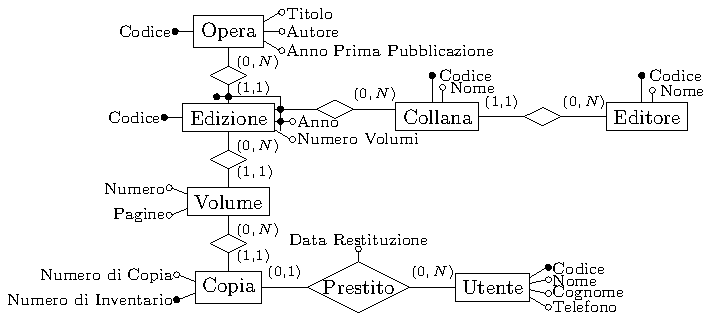
\includegraphics[scale=1.25]{schema_er_es_1.pdf}%
\end{figure}

\subsection{Esercizio 2}

Data la schematizzazione delle informazioni sulle automobili mostrate:
\begin{minted}[escapeinside=||]{c}
FIAT
    Corso Giovanni Agnelli 200-Torino
    www.fiat.it
    Modelli
        Panda
            Segmento: B
            Posti: 4
            Versioni:
                1.1 Cilindrata 1098 Prezzo 8.900
                1.2 4x4 Cilindrata 1250 Prezzo 13.000
                |\dots|        
        Punto
            Segmento: C
            Posti: 5
            Versioni:
                1.2 base Cilindrata 1212 Prezzo 11.100
                1.3 JT Cilindrata 1250 Prezzo 13.100
                |\dots|
        |\dots|
|\dots|
----------------------------------------------------
Segmenti
    A: super-compatte
    B: compatte
    C: medie
    D: grandi
    E: SW
\end{minted}

\subsubsection*{Domanda 1}


Definire uno schema concettuale (nel modello ER) che descriva la realtà di interesse; limitarsi agli aspetti che vengono espressamente mostrati, introducendo tutt'al più, 
ove lo si ritenga necessario, opportuni codici identificativi; mostrare le cardinalità delle relationship e gli identificatori delle entità:


Sono necessarie tre entità per la casa produttrice, per il modello prodotto e per la versione di un certo modello. Per ogni casa produttrice può non esistere un 
modello oppure un numero arbitrario di modelli. Analogamente per le versioni di un modello. Una casa produttrice può essere identificata sia dal 
codice e sia dal loro nome. Molti anni fa i modelli non erano registrati, mentre oggi i modelli hanno un nome registrato, quindi il loro nome è sufficiente per 
poterli identificare. 

Il segmento viene rappresentato tramite un'entità identificato da un codice, ed un attributo descrizione. Ogni modello deve essere legato ad un unico segmento tramite 
una relationship, e si può inserire un attributo posti. 

Le versioni hanno un nome, un prezzo, una cilindrata e possono essere identificati dal modello e dal nome, quindi si utilizza un identificatore esterno. 

\begin{figure}[H]%
    \centering%
    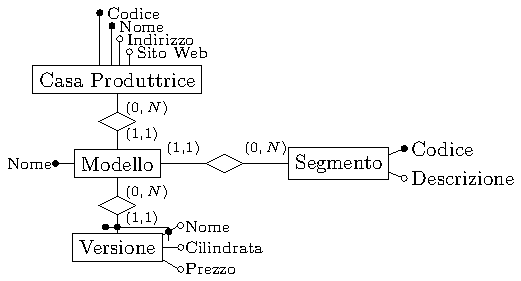
\includegraphics[scale=1.3]{schema_er_es_2.pdf}%
\end{figure}

\subsubsection*{Domanda 2}

Considerare le seguenti specifiche aggiuntive:
\begin{itemize}
    \item Per ogni versione è importante rappresentare le informazioni sui motori; ogni motore ha numero cilindri, cilindrata e potenza e uno stesso motore può essere 
utilizzato da più versioni (di uno stesso modello o anche di modelli diversi, ma dello stesso costruttore);
    \item \'{E} di interesse la storia dei prezzi: per ogni versione si deve riportare il prezzo attuale (con indicazione della data di ultimo aggiornamento) e i 
prezzi precedenti (ognuno con data di inizio e fine validità). 
\end{itemize}

Si aggiunge una nuova entità motore associata a modello con una relationship, identificato da un codice, con attributi numero di cilindrata cilindrata, da 
rimuovere dall'entità modello, e la potenza. Uno stesso motore può essere utilizzato da versioni diverse anche dello stesso modello, ma dello stesso costruttore, 
questo non si può rappresentare semplicemente quindi si inserisce come vincolo aggiuntivo a parole. 


Per rappresentare la storia dei prezzi si inserisce una cronologia delle versioni, ognuna associata ad un prezzo, si inserisce quindi un'entità 
chiamata ``versione con prezzo'', identificata dall'attributo data e la versione associata tramite relationship. Ha un attributo prezzo ed un 
attributo fine, con una cardinalità massima pari ad uno, che deve essere maggiore dell'attributo data. Quindi si deve togliere l'attributo prezzo 
dall'entità versione. 

\begin{figure}[H]%
    \centering%
    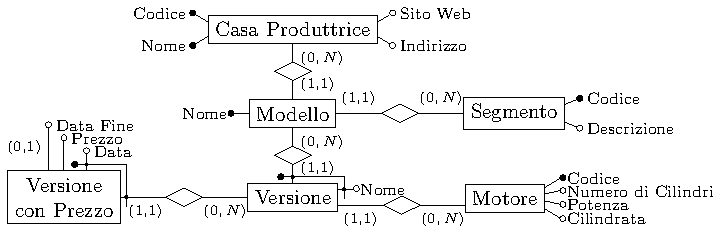
\includegraphics[scale=1.24]{schema_er_es_2_2.pdf}%
\end{figure}

\clearpage

\section{Esercizio dell'8 Novembre}

Considerare i quattro schemi seguenti:
\begin{figure}[H]%
    \centering%
    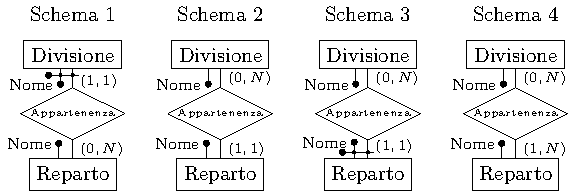
\includegraphics[scale=1.4]{domanda_8-11-24.pdf}%
\end{figure}

Rispondere alle domande seguenti con un sì o un no nella casella:
\begin{center}
    \begin{tabular}{|c|c|c|c|c|}
        \hline
        & S. 1 & S. 2 & S. 3 & S. 4\\
        \hline
        Possono esistere due divisioni con lo stesso nome, in reparti diversi? & Sì & No & No & No\\
        \hline
        Possono esistere due reparti con lo stesso nome, in divisioni diverse? & No & No & Sì & No\\
        \hline
        Possono due divisioni appartenere ad uno stesso reparto? & Sì & No & No & Sì\\
        \hline
        Possono due reparti appartenere alla stessa divisione? & No & Sì & Sì & Sì\\
        \hline        
    \end{tabular}
\end{center}

\begin{enumerate}
    \item Negli ultimi tre schemi la divisione viene identificata univocamente dal nome, quindi non è possibile. Al contrario per il primo schema dove una divisione viene identificata dal proprio nome e dall'appartenenza ad un reparto. 
    \item Per il terzo schema, un reparto viene identificato sia dal nome che dall'appartenenza ad una certa divisione quindi è possibile. Per tutti gli altri schemi invece ciò non è possibile poiché sono identificati unicamente dal loro nome. 
    \item Per gli schemi due e tre questo non è possibile poiché la cardinalità della relationship non permette l'appartenenza di più di una divisione ad un reparto. Negli schemi uno e quattro invece è possibile poiché la cardinalità è uno a molti, la prima, e molti a molti, la seconda. 
    \item Per gli ultimi tre schemi questo è possibile poiché la cardinalità è sempre molti ad uno o a molti, per l'entità ``Divisione''. Mentre nel primo schema può avere solo un'appartenenza a reparto. 
\end{enumerate}


\clearpage

\section{Esercitazione del 18 Novembre}

\subsection{Domanda 1}

Mostrare lo schema concettuale per una base di dati per il programma di una stazione presso un teatro, secondo le seguenti specifiche:
\begin{itemize}
    \item Ogni concerto ha un codice, un titolo ed una descrizione, ed è costituito da un insieme di pezzi musicali. 
    \item Ogni pezzo ha un codice, un titolo ed un autore (con codice e nome); uno stesso pezzo può essere rappresentato in diversi concerti. 
    \item Ogni concerto è eseguito da un'orchestra; ogni orchestra ha un nome, un direttore (del quale interessano solo nome e cognome) e un insieme di orchestrali. 
    \item Ogni orchestrale ha una matricola (univoca nell'ambito della base di dati), nome e cognome, e può partecipare a più orchestre, in ciascuna delle quali suona un solo strumento, ma in orchestre diverse può suonare strumenti diversi. 
    \item Ogni concerto è tenuto più volte, in giorni diversi, ma sempre nella stessa sala. 
\end{itemize}

Si può cominciare sia dall'entità concerto, ogni concerto è costituito da un insieme di pezzi musicali, per cui si ha una relazione con l'entità 
pezzo. Ogni concerto viene eseguito da un'orchestra quindi si inserisce un'entità orchestra. Ogni concerto ha un attributo codice e nome. 
Serve un'entità che identifica l'autore, ma è presente anche la persona orchestrale, si vuole rappresentare generalmente con l'entità musicista. Questa entità viene 
connessa all'entità pezzo con una relazione ``Autore''. Si può inserire un'entità direttore, in relazione ad orchestra, ma potrebbe essere 
identificato da un attributo, poiché non vengono specificate altre proprietà significative. L'entità orchestra viene connessa all'entità orchestrale. 
Ogni pezzo ha un singolo autore, ed ogni autore può scrivere più pezzi, quindi si ha una cardinalità uno a molti, quindi non può essere 
inserito come attributo. Ogni pezzo potrebbe avere più di un autore, ma in questo contesto viene specificato un singolo autore. La relazione tra 
pezzi e concerti è molti a molti, poiché ogni concerto è un insieme di pezzi, anche uguali tra di loro. 
Ogni orchestro viene eseguito da una singola orchestra, quindi si ha una cardinalità uno a molti, così come con direttore. 
Ogni orchestrale ha una matricola univoca nella base di dati, l'identificatore della relazione. Si può inserire lo strumento come l'attributo della 
relazione tra orchestra ed orchestrale. Se si volessero rappresentare caratteristiche dello strumento, non basterebbe come attributo, e 
bisognerebbe promuovere la relazione tra orchestrale ed orchestra ad entità partecipazione. A questa entità si può includere l'attributo 
strumento, ma per ottenere lo stesso effetto della relationship, bisogna includere un identificatore, la doppia identificazione esterna, costituita 
dalla relazione ad orchestra ed orchestrale. In caso si vuole aggiungere le proprietà dello strumento si può aggiungere queste entità senza problemi. 

Si inserisce l'entità sala con attributi codice, nome e capienza. Ma la data di ogni concerto non si può inserire come attributo sulla relazione o 
sull'entità concerto. Si inserisce quindi un'ulteriore relazione ad un'entità evento, con attributo data all'entità concerto. Questo viene identificato 
dalla data e dall'entità concerto in relazione. 

\begin{figure}[H]%
    \centering
    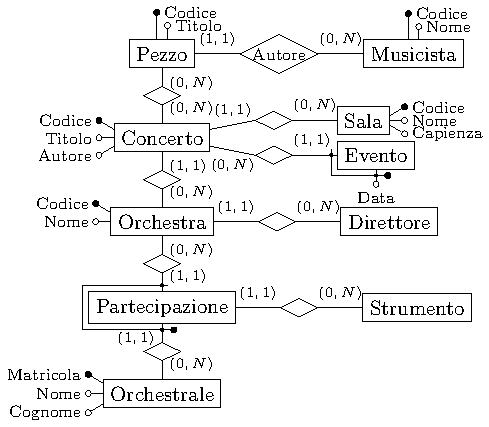
\includegraphics[scale=1.25]{schema_er_es_3.pdf}%
\end{figure}

\subsection{Domanda 2}

Modificare lo schema prodotto in risposta alla domanda precedente con riferimento alle seguenti specifiche che modificano le precedenti 
(mostrare l'intero schema modificato):
\begin{itemize}
    \item Interessa il programma di concerti di diversi teatri (e non di un solo teatro come nella domanda precedente); per ogni teatro sono rilevanti un codice, il nome e l'indirizzo. 
    \item Per ogni concerto, interessa anche l'ordine dei pezzi ed è anche possibile che un pezzo venga ripetuto più volte nello stesso concerto. 
    \item I direttori (che dirigono ciascuno al massimo una orchestra) possono essere anche orchestrali (nella stessa orchestra che dirigono o in altre). 
    \item Ogni orchestrale suona un solo strumento, lo stesso in tutte le orchestre cui partecipa.
    \item Ogni concerto è tenuto più volte, in giorni diversi, non necessariamente sempre nella stessa sala. 
\end{itemize}

Se il concerto può avvenire in sale diverse allora bisogna legare l'entità sala all'entità evento. E per indicare che ogni orchestrale suona un unico 
strumento bisogna legare strumento direttamente ad orchestrale. 
Si può generalizzare orchestrale e direttore come sottoinsieme di un'altra entità artista con matricola, nome e cognome, mantenendo le relazioni 
invariate. 

Per inserire una posizione ai pezzi, non si può inserire un attributo alla relazione poiché potrebbe avere più posizioni in un concerto, si promuove 
quindi ad entità questa relazione chiamata ``Pezzo in Scaletta''. Questo ha un attributo posizione, con un identificatore esterno con posizione e la 
relazione concerto. 

Inoltre bisogna inserire un'entità teatro in relazione con concerto. Questa tuttavia deve essere legata a sala e deve essere comunque legata agli 
eventi. Si crea in questo modo un ciclo e bisogna inserire un ulteriore vincolo non rappresentabile nello schema ER. Altrimenti non bisogna legare teatro e concerto tramite una relationship. 


\begin{figure}[H]%
    \centering%
    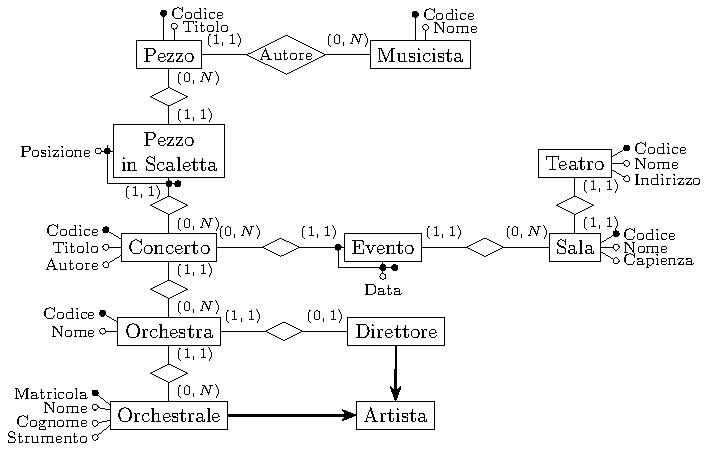
\includegraphics[scale=1.25]{schema_er_es_4.pdf}%
\end{figure}

\clearpage

\section{Esercitazione del 25 Novembre}

\subsection{Esercizio 1}

Si considera il modello ER seguente:
\begin{figure}[H]%
    \centering%
    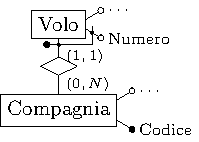
\includegraphics[scale=1.25]{schema_voli_25-11-24_2.pdf}%
\end{figure}

Rappresentare un modello logico corrispondente. \\
Si considera l'entità compagnia per prima, dato che non ha identificatori esterni, come una relazione con chiave codice e diversi 
attributi. Mentre l'entità volo si realizza come una relazione, dove la chiave è composta dal numero di volo e la compagnia di appartenenza del 
volo, con un vincolo di integrità referenziale tra l'attributo codice e la relazione compagnia.  
\begin{itemize}
    \item Compagnia(\underline{Codice}, $\cdots$)
    \item Volo(\underline{Codice}, \underline{Numero}, $\cdots$)
\end{itemize}

\subsection{Esercizio 2}

Analogamente per questo schema ER:

\begin{figure}[H]%
    \centering%
    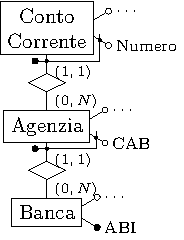
\includegraphics[scale=1.25]{schema_banca_25-11-24.pdf}%
\end{figure}

Si rappresenta con una relazione banca, con chiave ABI; una relazione agenzia con chiave ABI e CAB con vincolo di integrità referenziale tra 
il suo attributo ABI e la relazione banca; una relazione conto corrente con chiave ABI, CAB e numero di conto, con un vincolo di integrità 
referenziale tra ABI e banca e CAB e agenzia
\begin{itemize}
    \item Banca(\underline{ABI}, $\cdots$)
    \item Agenzia(\underline{ABI}, \underline{CAB}, $\cdots$)
    \item CC(\underline{ABI}, \underline{CAB}, \underline{NUM}, $\cdots$)
\end{itemize}

Ci sono alcuni casi nei quali l'identificazione esterna ha un significato particolare e necessario. 

\subsection{Esercizio 3}

Si considera questo schema concettuale:

\begin{figure}[H]%
    \centering%
    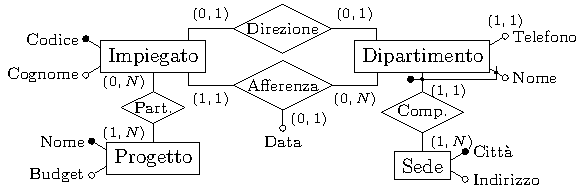
\includegraphics[scale=1.25]{schema_azienda_25-11-24.pdf}%
\end{figure}

Si comincia dalle entità senza identificazione esterna. Partendo dall'entità impiegato, si crea una relazione impiegato con una chiave codice, 
ed un attributo cognome. Analogamente per le entità progetto e sede. L'entità dipartimento ha un identificatore esterno composto dal nome del dipartimento e 
la partecipazione alla relationship composizione, la sua chiave è composta dall'attributo nome e la chiave dell'entità sede. Si deve utilizzare una tabella 
per rappresentare la relationship partecipazione, con una chiave data dalla chiave delle due relazioni che identificano le due entità. Su questi 
due attributo c'è un vincolo di integrità referenziale con le relazioni impiegato e progetto. Inoltre è presente un vincolo 
di integrità referenziale tra dipartimento e sede sull'attributo città. Per rappresentare la relationship uno a molti tra impiegato e 
dipartimento si inserisce l'attributo nome dipartimento e città, con un vincolo di integrità referenziale con la chiave di dipartimento. Si 
inseriscono questi attributo all'0interno della relazione impiegato, poiché se fossero presenti dentro dipartimento, sarebbero presenti 
più valori di impiegato, mentre un impiegato afferisce ad un singolo dipartimento, ed è possibile rappresentarlo senza tabelle aggiuntive. 
La relationship afferenza ha anche un attributo data con una cardinalità minima zero, quindi dovrà poter ammettere valori nulli, al contrario 
degli altri attributi descritti, nella relazione impiegato. Poiché la relationship direzione ha una cardinalità massima pari ad uno, si potrete 
inserire come attributo all'interno di impiegato e dipartimento. Conviene scegliere l'opzione più intuitivamente sensata, quindi si inserisce dentro 
la relazione dipartimento, poiché è più corretto dato che rappresenta una proprietà di dipartimento più di una proprietà di impiegato. 

\begin{itemize}
    \item Impiegato(\underline{Codice}, Cognome, Data Afferenza*)
    \item Progetto(\underline{Nome}, Budget)
    \item Sede(\underline{Città}, Indirizzo)
    \item Dipartimento(\underline{Nome}, \underline{Città}, Telefono, Direttore*)
    \item Partecipazione(\underline{Progetto}, \underline{Impiegato})
\end{itemize}

\subsection{Esercizio 4}

Si considera questo schema simile al precedente, ma con un identificatore esterno sull'entità sede, invece che sull'entità dipartimento. 

\begin{figure}[H]%
    \centering%
    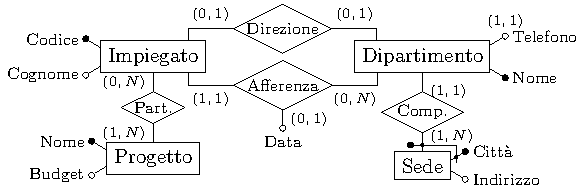
\includegraphics[scale=1.25]{schema_azienda_25-11-24_2.pdf}%
\end{figure}

In questo caso la relazione dipartimento viene identificata solamente da nome. Mentre per quanto riguarda sede, ha il nome del dipartimento e 
città come chiave, con un vincolo di integrità referenziale sull'attributo nome del dipartimento con la relazione. Inoltre l'attributo impiegato 
ha solo l'attributo dipartimento con un vincolo di integrità referenziale con la relazione dipartimento. In caso ogni impiegato possa essere 
direttore di un unico dipartimento non sarebbe un vincolo esprimibile, ma si potrebbe rappresentare questo attributo come chiave per la 
relazione dipartimento, ma in caso fossero presenti due dipartimenti con lo stesso direttore questo non funzionerebbe. 

\begin{itemize}
    \item Impiegato(\underline{Codice}, Cognome, Data Afferenza*)
    \item Progetto(\underline{Nome}, Budget )
    \item Sede(\underline{Nome Dipartimento}, \underline{Città}, Indirizzo )
    \item Dipartimento(\underline{Nome}, Telefono, Direttore)
    \item Partecipazione(\underline{Progetto}, \underline{Impiegato})
\end{itemize}

\subsection{Esercizio 5}

Con riferimento a ciascuno dei seguenti schemi concettuali mostrare una base di dati relazionale ottenuta per traduzione del 
modello ER, che evidenzi le caratteristiche dello schema. Per ciascuna relazione, mostrare anche solo poche ennuple, che 
evidenzino appunto le caratteristiche interessanti. Indicare in qualunque modo, purché comprensibile, 
anche i vincoli di chiave e di integrità referenziale. 

\begin{figure}[H]%
    \centering%
    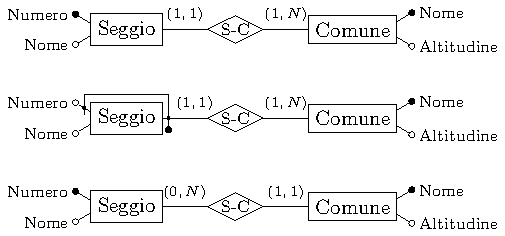
\includegraphics[scale=1.25]{schema_elezioni_25-11-24.pdf}%
\end{figure}

Per lo schema A si ha una relazione seggio con chiave numero, attributo nome e comune con un vincolo di integrità referenziale con la chiave nome 
della relazione comune, con un altro attributo altitudine. 
\begin{center}
    \begin{tabular}{|c|c|c|}
        \hline 
        \underline{Numero} & Nome & Comune\\
        \hline
        1 & x & Castello\\
        \hline
        2 & y & Riva\\
        \hline
        3 & z & Riva\\
        \hline
    \end{tabular}
    \begin{tabular}{|c|c|}
        \hline
        \underline{Nome} & Altitudine\\
        \hline
        Castello & 300\\
        \hline
        Riva & 200\\
        \hline
    \end{tabular}
\end{center}
Il caso B a differenza del caso A ha la chiave primaria di seggio composta da numero e comune, mentre i vincoli e la struttura della relatone 
comune sono invariati. 
\begin{center}
    \begin{tabular}{|c|c|c|}
        \hline 
        \underline{Numero} & Nome & \underline{Comune}\\
        \hline
        1 & x & Castello\\
        \hline
        2 & y & Riva\\
        \hline
        1 & z & Riva\\
        \hline
    \end{tabular}
    \begin{tabular}{|c|c|}
        \hline
        \underline{Nome} & Altitudine\\
        \hline
        Castello & 300\\
        \hline
        Riva & 200\\
        \hline
    \end{tabular}
\end{center}
In questo caso nei dati si inserisce un seggio con lo stesso numero, ma in un comune differente per mostrare che si identificano seggi per lo 
stesso numero, nello stesso comune. 

Nel caso C la relationship è invertita, e la relazione seggio contiene solamente la chiave numero ed il suo nome, mentre la relazione comune 
contiene anche un attribuito seggio con un vincolo di integrità referenziale con la chiave della relazione seggio. 
\begin{center}
    \begin{tabular}{|c|c|}
        \hline 
        \underline{Numero} & Nome \\
        \hline
        1 & x \\
        \hline
        2 & y \\
        \hline
        3 & z \\
        \hline
    \end{tabular}
    \begin{tabular}{|c|c|c|}
        \hline
        \underline{Nome} & Altitudine & Seggio\\
        \hline
        Castello & 300 & 1\\
        \hline
        Riva & 200 & 2\\
        \hline
    \end{tabular}
\end{center}

\subsection{Esercizio 6}

Mostrare uno schema concettuale per una realtà i cui dati siano organizzati per mezzo del seguente schema relazionale:
\begin{itemize}
    \item Nazioni(\underline{Codice}, Nome);
    \item Compagnie(\underline{Codice}, Nome, Nazione), con un vincolo di integrità referenziale fra l'attributo nazione e la relazione nazioni;
    \item Aeroporti(\underline{Codice}, Nome, Città), con un vincolo di integrità referenziale fra città e la relazione città;
    \item Città(\underline{Codice}, Nome);
    \item Voli(\underline{Compagnia}, \underline{Numero}, Aeroporto Partenza, Aeroporto Arrivo, Ora Partenza Prevista, Ora Arrivo Previsto, Tipo Aeromobile), con vincoli 
    di integrità referenziale tra compagnia e la relazione compagnie, aeroporto partenza e aeroporti, aeroporto arrivo e aeroporti, e tipo aeromobile con tipo aeromobili;
    \item VoliEffettivi(\underline{Compagnia}, \underline{Numero}, \underline{Data}, Ora Partenza Effettiva, Ora Arrivo Effettivo), un vincolo di integrità referenziale fra compagnia e numero e la relazione voli;
    \item TipoAeroMobile(\underline{Codice}, Nome).
\end{itemize}

Si comincia dalle entità senza vincoli di integrità referenziale. Si comincia dal'entità nazioni, in relazione con compagnie. Analogamente l'entità 
città in relazione con aeroporto, ed i relativi attributi per queste entità. Si inserisce l'entità tipo aeromobile con i relativi attributi non 
ancora legata con relationship. Un relazione rappresenta una relationship quando contiene due attributi come chiavi, in vincoli di integrità 
referenziale con due relazioni diverse, poiché le uniche relationship che generano una tabella separata sono quelle molti a molti. Si hanno due 
relazioni tra volo ed aeroporto per gli aeroporti di partenza e di arrivo. Inoltre si ha una relationship tra l'entità volo e 
compagnie con un identificatore esterno sulla compagnia e l'attributo numero del volo. 

\begin{figure}[H]%
    \centering%
    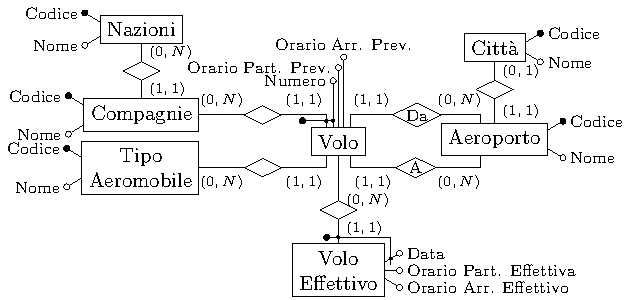
\includegraphics[scale=1.25]{schema_voli_25-11-24.pdf}%
\end{figure}

\subsection{Esercizio 7}

Considerare lo schema concettuale seguente:
\begin{figure}[H]%
    \centering
    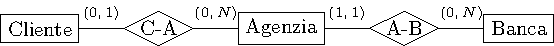
\includegraphics[scale=1.25]{schema_es_7_25-11-24.pdf}%
\end{figure}

Vallare la convenienza dell'introduzione di una relationship C-B fra Cliente e Banca. Tale relationship è ridondante in quanto derivabile dalla 
concatenazione  delle relationship esistenti. Considerare un carico applicativo che includa come operazioni principali le leggenti:
\begin{itemize}
    \item Ricerca delle Banche di un Cliente, di uci è dato il codice, con frequenza $f_!=200$;
    \item Inserimento di una nuova occorrenza della relationship C-A, dati i codici identificativi di Cliente e Agenzia, assumendo 
    per semplicità che le occorrenze di Cliente e Agenzia siano già nella base di dati, e che il Cliente non 
    abbia ancora legami né con l'Agenzia n* con la relativa Banca, con frequenza $f_2=10000$. 
\end{itemize}

Considerare i costi delle letture e scritture delle entità e della relationship molti a molti, ignorando quelli della relationship uno a molti e 
considerare il costo delle scritture doppio di quello delle letture. Assumere che ogni Cliente abbia rapporti, relationship C-A, mediamente con $k=10$ Agenzie. 

In generale la ridondanze aumenta le prestazioni in lettura, ma la peggiore in scrittura. 

Il costo complessivo è dato da $c_1f_2+c_2f_2$, dove il costo della prima operazione si ottiene con la ridondanza pari ad una singola lettura di 
costo $k=10$, mentre senza ridondanza bisogna effettuare tre letture con un costo $3k=30$. 
Mentre per la seconda operazione con la ridondanza bisogna effettuare una lettura per verificare l'occorrenza ed in caso inserirla con due 
scritture di costo $5$, mentre senza ridondanza è sufficiente una singola scrittura con costo $2$. 
Si ha quindi:
\begin{gather*}
    c_{\mathrm{r}}=10\cdot200+5\cdot10000=52000\\
    c_{\mathrm{s}}=30\cdot200+2\cdot10000=26000\\
    c_{\mathrm{r}}>c_{\mathrm{s}}\tageq
\end{gather*}
Quindi non è conveniente avere ridondanza. 

\clearpage

\section{Esercitazione del 29 Novembre}

\subsection{Esercizio 1}

Progettare lo schema della base di dati relazionale per gestire i dati della realtà descritta dallo schema concettuale in figura:
%% TODO img ex 1 compito B 25 gen 2018
% \begin{figure}[H]%
%     \centering%
%     \includegraphics{}%
% \end{figure}

Si comincia dall'entità nazione senza identificatori esterni, come relazione con con gli stessi attributi e chiave CN. L'entità città rappresenta una 
relazione con chiave CC e CN con un vincolo di integrità referenziale con nazione. La relationship C-N è già implicitamente descritta 
da queste due relazioni. Si segue con l'entità istituzione, con una relationship uno a molti con città, ogni istituzione ha una sola 
sede per ogni città, quindi si ha un vincolo di integrità referenziale tra la chiave di città e gli attributi CC e CN di istituzione. Si passa 
all'entità persona con affiliazione, senza attributi, ma un identificatore esterno sia con istituzione che con città. Si inserisce quindi 
la relazione persona, con un codice chiave ed un nome, la relazione persona con affiliazione ha come chiave persona ed istituzione, con un vincolo di 
integrità referenziale alle chiavi di persona ed istituzione. Questo schema rappresenta una ristrutturazione, per permettere questa traduzione, 
infatti quest'entità persona con affiliazione poteva essere uan generalizzazione di persona. Si procede con l'entità sessione, questa è collegata 
da una relazione molti a molti con persona con affiliazione, quindi è necessaria un'altra relazione chiamata intervento. 
Si ha un'entità convegno con un'identificatore esterno con l'entità serie tramite la relazione S-C, quindi si inserisce prima quest'ultima 
relazione. Dentro la relazione sessione va inserita anche la chiave di convegno. La relazione convegno ha attributi data, chiave anno e codice serie, 
ed attributi codice città e codice nazione, con un vincolo di integrità referenziale con la città e nazione. La relazione serie ha una chiave codice, 
un titolo, ed un attributo materia, vincolo di integrità referenziale con la relazione materia. Questa relazione ha chiave codice e attributo 
materia. 

\begin{itemize}
    \item Nazione(\underline{CN}, Nazione);
    \item Città(\underline{CC},\underline{CN});
    \item Istituzione(\underline{Codice}, Nome, Città, Nazione);
    \item Persona(\underline{Codice}, Nome);
    \item Persona Con Affiliazione(\underline{Persona}, \underline{Istituzione})
    \item Sessione(\underline{Codice}, Titolo, Ora);
    \item Intervento(\underline{Sessione}, \underline{Persona}, \underline{Istituzione});
    \item Convegno(Data, \underline{Anno}, \underline{Serie}, Città, Nazione)
    \item Serie(\underline{Codice}, Titolo, Materia)
    \item Materia(\underline{Codice}, Materia)
\end{itemize}

\subsection{Esercizio 2}

Con riferimento all'esercizio precedente, per le due porzioni di schema in figura mostrare le tabelle risultati dalla progettazione logica con 
alcune istanze(ennuple):
% \begin{figure}[H]%
%     \centering%
%     \includegraphics{}%
% \end{figure}

%% TODO fare prima parte ex

Si considerano le tabelle corrispondenti alla relazioni del secondo schema:
\begin{center}
    \begin{tabular}{|c|c|}
        \hline
        \multicolumn{2}{|c|}{Istituzione}\\
        \hline
        \underline{Codice} & Nome\\
        \hline
        1 & A\\\hline 2&B\\\hline 3&C\\\hline
    \end{tabular}
    \begin{tabular}{|c|c|}
        \hline
        \multicolumn{2}{|c|}{Persona}\\
        \hline
        \underline{Codice}& Nome\\
        \hline
        00&Anna\\\hline 01&Lino\\\hline 02&Bob\\\hline 03&Eric\\\hline 04 & Sam\\\hline
    \end{tabular}
    \begin{tabular}{|c|c|}
        \hline
        \multicolumn{2}{|c|}{Persona con Aff.}\\
        \hline
        \underline{Persona} & \underline{Istituzione}\\
        \hline
        00&1\\\hline 01 & 1\\\hline 02&2\\\hline 00&2\\\hline
    \end{tabular}
\end{center}

\subsection{Esercizio 3}

%% 25 gen 2018 A

Lo schema concettuale seguente rappresenta un insieme di corsi ed un insieme di iscrizioni a tali cosi. ello schema l'attributo ricavo è 
ridondante, poiché può essere ottenuto moltiplicando il costo del corso per il numero di iscritti, cioè il prodotto del valore dell'attributo costo di ogni 
occorrenza dell'entità corso per il numero di occorrenze dell'entità persona a cui essa è correlata tramite la relationship iscrizione:
% \begin{figure}[H]%
%     \centering%
%     \includegraphics{}%
% \end{figure}

Valutare se convenga o meno mantenere la ridondanza, assumendo corso abbia $C_c=1000$ occorrenze, persona ne abbia $C_p=3000$ ed iscrizione 
$C_i=30000$, e quindi che ogni corso abbia mediamente $C_{ci}=30$ iscritti, e che il carico applicativo includa le operazioni principali seguenti:
\begin{itemize}
    \item Calcolo del ricavo di un corso, dato il codice, con frequenza $f_1=50$;
    \item Iscrizione di una persona, già nella base di dati e di cui è dato il codice fiscale, ad un corso, di cui è dato il codice, con 
    frequenza $f_2=20000$, in sostanza, questa operazione richiede l'inserimento di un'occorrenza di iscrizione. 
\end{itemize}

Considerando i costi delle letture e scritture delle occorrenze e considerare il costo delle scrittura pari a quello delle letture. 


La prima operazione con ridondanza consiste in una singola lettura sulla relazione corso, la seconda operazione consiste in una 
lettura e scrittura su corso ed una scrittura su iscrizione. Il costo totale delle operazioni con ridondanza è quindi:
\begin{equation*}
    C=c_1\cdot f_1+c_2\cdot f_2=1_{\mathrm{r}}\cdot50+(1_{\mathrm{r}}+2_{\mathrm{w}})\cdot20000=60050
\end{equation*}
Senza ridondanza è necessario oltre alla lettura su corso per conoscere il costo, leggere tutte le 30 occorrenze di iscrizione. Nella seconda operazione, 
è sufficiente inserire l'occorrenza in iscrizione:
\begin{equation*}
    C=c_1\cdot f_1+c_2\cdot f_2=(1_{\mathrm{r}}+30_\mathrm{r})\cdot50+1_\mathrm{w}\cdot20000=21550
\end{equation*}

Quindi non è conveniente avere ridondanza. 

\subsection{Esercizio 4}

%% TODO 7 feb 2017 compito A ex 3

%% alternativa alla generalizzazione con relazione e identificatore esterno tra dipendente e professore 

\end{document}